\pdfminorversion=3
\documentclass[tikz]{standalone}
\usepackage{schemabloc}
%\usepackage{vuiprepstandalone}
%\usepackage{alain2}

\begin{document}
\footnotesize

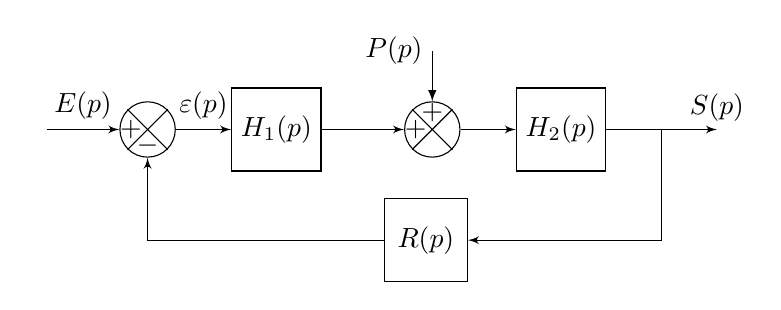
\begin{tikzpicture}
\sbEntree{E}

\sbComp{c1}{E}
    \sbRelier[$E(p)$]{E}{c1}

\sbBloc{b1}{$H_1(p)$}{c1}
    \sbRelier[$\varepsilon(p)$]{c1}{b1}
    
\sbSumh{c2}{b1}
    \sbRelier{b1}{c2}

\sbBloc{b2}{$H_2(p)$}{c2}
    \sbRelier{c2}{b2}
    

\sbSortie[4]{S}{b2}
    \sbRelier{b2}{S}
    \sbNomLien[0.8]{S}{$S(p)$}

\sbDecaleNoeudy[4]{S}{U}
\sbDecaleNoeudx[-7]{U}{U2}
\sbBlocr{r}{$R(p)$}{U2}
\sbRelieryx{b2-S}{r}
\sbRelierxy{r}{c1}
%\sbRenvoi{b2-S}{c1}{}

\draw [latex-] (c2) --++ (0,1) node[left] {$P(p)$};

\end{tikzpicture}

\normalsize
\end{document}